\chapter{Failure criteria}\label{ch2:title}

Failure criteria aim to describe in the most accurate way rock failure. The most successful criteria are a usually a generalization of experiments results, from a combination of axisymmetric and multi-axial tests. Indeed, failure criteria are a theoretical conjecture aimed to describe what is observed from material behavior. In this chapter, a presentation of the mathematical formulation of selected criteria is provided. The theory presented is based on the work of Labuz (2018) [1] and Folta (2016) [2], in which detailed descriptions of the failure criteria can be found.

\section{Background on failure criteria}

Failure criteria are a theoretical derivation of a fundamental mathematical function that describe rock failure: 

\begin{equation}\label{eq2:rockfail}
    f\left(\sigma_{x x}, \sigma_{y y}, \sigma_{z z}, \sigma_{x y}, \sigma_{y z}, \sigma_{z x}\right)=\text { constant }
\end{equation}

This function is expressed in terms of $\sigma_{ij}$ the stresses  acting on the rock.  Equation \ref{eq2:rockfail} can be simplified in the case of iso

tropic material analysis. Indeed, the isotropic rock strength properties are the same in all directions, which leads to a directional independence of the stress state. The fundamental function can then be written as follow: 

\begin{equation}\label{eq2:fsigconst}
    f\left(\sigma_{I}, \sigma_{II}, \sigma_{III} \right)=\text { constant }
\end{equation}

$\sigma_{I}$, $\sigma_{II}$ and $\sigma_{III}$ being the three principal stress acting on the rock, respectively major, intermediate and minor stress. 

In order to emphasize on the directional independence of the stress state, the failure criteria can be formulated within the framework of the stress invariants. The fundamental mathematical formulation then becomes:

\begin{equation}\label{eq2:fijjconst}
    f\left(I_{I}, J_{II}, J_{III} \right)=\text { constant }
\end{equation}

$I_{I}$is the first invariant of the stress tensor $\sigma_{ij}$ and $J_{II}$, $J_{III}$ the second and third invariants of the deviatoric stress tensor  : 

\begin{align}
   I_1 &= \sigma_{I} + \sigma_{II} + \sigma_{III} \\
   J_{2}&=\frac{1}{6}\left[\left(\sigma_{I}-\sigma_{I I}\right)^{2}+\left(\sigma_{I I}-\sigma_{I I I}\right)^{2}+\left(\sigma_{I I I}-\sigma_{I}\right)^{2}\right]\\
   J_{2}&=\left(\sigma_{I}-p\right)\left(\sigma_{I I}-p\right)\left(\sigma_{III}-p\right)
\end{align}

From these invariants, three others can be defined, and will be used in this thesis: the mean stress $p$ , the deviatoric stress $q$ and the Lodge angle $\theta$ . Failure criteria are then described by:

\begin{equation} \label{eq2:fpqtconst}
    f(p,q,\theta) = \text{constant}
\end{equation}

\begin{equation} \label{eq2:peq}
    p=\frac{I_{1}}{3}=\frac{\sigma_{I}+\sigma_{M}+\sigma_{III}}{3}
\end{equation}

\begin{equation}\label{eq2:qeq}
    q=\sqrt{3 J_{2}}=\frac{1}{6} \sqrt{\left[\left(\sigma_{I}-\sigma_{II}\right)^{2}+\left(\sigma_{II}-\sigma_{III}\right)^{2}+\left(\sigma_{III}-\sigma_{I}\right)^{2}\right]}
\end{equation}

\begin{equation}\label{eq2:theta}
    \theta=\frac{1}{3} \arccos \left(\frac{3 \sqrt{3}}{2} \frac{J_{3}}{J_{2}^{3 / 2}}\right)=\arctan \left[\frac{\sqrt{3}\left(\sigma_{M}-\sigma_{M}\right)}{2 \sigma_{I}-\sigma_{I I}-\sigma_{M I}}\right]
\end{equation}

The Lodge angle is a measure of the stress state: $0^{\circ} \leq \theta \leq 60^{\circ}$ , particularly $\theta = 0^{\circ}$  for axisymmetric compression $\sigma_{II} = \sigma_{III} $ and $\theta = 60^{\circ}$ in the case of axisymmetric extension ($\sigma_{II} = \sigma_{I} $). 

Equations \ref{eq2:fsigconst}, \ref{eq2:fijjconst} and \ref{eq2:fpqtconst} unveils the three-dimensional nature of the failure envelop and consequently of failure criteria. Indeed, depending on the state of stress ordering, failure criteria describe six planes, or failure surfaces, in a three-dimensional $\sigma_1 -\sigma_2 -\sigma_3$  space. For instance, a linear criterion, written in terms of the three principal stresses, shows a pyramidal failure envelop of which the planes have a common vertex $V_0$ , the theoretical isotropic tensile strength, on the tension side of the space. This example is presented in Fig \ref{fig2:pyramid}a.  

\begin{figure}[tb]
    \centering
    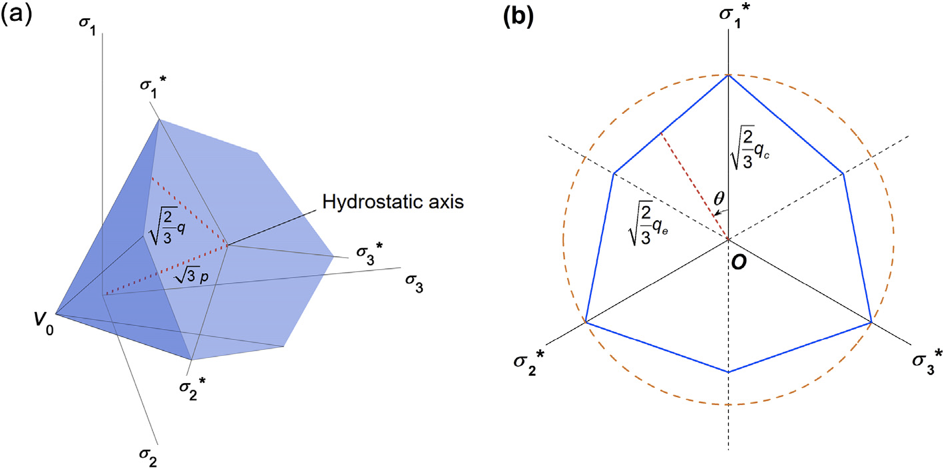
\includegraphics[width=\columnwidth]{ch2/pyramid.png}
    \caption{Failure surface in (a) the principal stress space and (b) the $\pi$-plane \cite[Labuz 2018]{Labuz2018}}
    \label{fig2:pyramid}
\end{figure}

However, although the three-dimensional representation of the failure envelop is the most complete, it is not the most practical to use and to show. Therefore, two-dimensional coordinates systems are preferred, as the  $(\sigma_3 -\sigma_1)$plane, the  $(p-q)$ plane and the $\pi$-plane.  

The $\pi$-plane. is a section of the failure envelop in the principal stress space, perpendicular to the hydrostatic axis. It is also called the equipressure plane, as the mean stress is constant over the plane. Moreover, the axes $(\sigma_1^*,\sigma_2^*,\sigma_3^*)$ are the projection of the coordinate axis on the $\pi$-plane (cf. \ref{fig2:pyramid}b.). Each point on in the principal stress space can be represented in polar coordinates in this plane. As the mean stress is constant over the $\pi$-plane, the point is at a distance $r$ from the origin of the hydrostatic axis and oriented at the Lodge angle $\theta$ from the  $\sigma_1^*$ axis. Then the principal coordinates of the same point on the $\pi$-plane can be written as: 

\begin{align}
    \sigma_1 &= p + \frac{\sqrt{6}}{3}r\cos\left(\theta\right) \label{eq2:sig1}\\
    \sigma_2 &= p + \frac{\sqrt{6}}{3}r\sin\left(\frac{\pi}{6}+\theta\right)\\
    \sigma_3 &= p + \frac{\sqrt{6}}{3}r\sin\left(\frac{\pi}{6}-\theta\right) \label{eq2:sig3}
\end{align}

In the next sections, selected failure criteria will be presented along with their formulation in each coordinates system. 

\section{Mohr-Coulomb criterion}

The Mohr-Coulomb failure criterion (MC) is the most popular and widely used criterion. In its original formulation, it describes the shear strength of a material as a function of the normal stress $\sigma$ , and two material parameters known as the internal failure angle $\theta$ and the cohesion $c$ :

\begin{equation}
    \tau = \sigma \tan \phi + c
\end{equation}

This criterion was developed considering failure of isotropic materials without taking into account the intermediate stress effect. It can be written in terms of the major and minor stresses: 

\begin{equation}
    \tau = \frac{\sigma_I - \sigma_{III}}{2} \cos \phi
\end{equation}

\begin{equation}
    \sigma = \frac{\sigma_I + \sigma_{III}}{2} - \frac{\sigma_I - \sigma_{III}}{2} \sin \phi
\end{equation}

Then in its final form:

\begin{equation} \label{eq2:MCfinalform}
    \sigma_{I}=\frac{1+\sin \phi}{1-\sin \phi} \sigma_{I I I}+\frac{2 c \cos \phi}{1-\sin \phi}
\end{equation}

or

\begin{equation}\label{eq2:MCcondenseform}
    \sigma_I = K_p \sigma_{III} + C_0
\end{equation}

where $K_p$ is the slope of the failure surface in $(\sigma_3 -\sigma_1)$plane and $C_0$ is the uniaxial compression strength of the rock. 

\subsection{Mohr-Coulomb in the \texorpdfstring{$(\sigma_3 -\sigma_1)$}{sigma 3 - sigma 1} plane}

Fig \ref{fig2:mc_sig1sig3} present the graphical construction of MC envelop in the $(\sigma_3 -\sigma_1)$ plane. The common vertex of the failure surfaces in extension and compression can be expressed using $\sigma_I = \sigma_{III} = -V_0$ :

\begin{equation}\label{eq2:MC_Vo}
    V_0 = \frac{C_0}{K_p-1}
\end{equation}


\begin{figure}[tb]
    \centering
    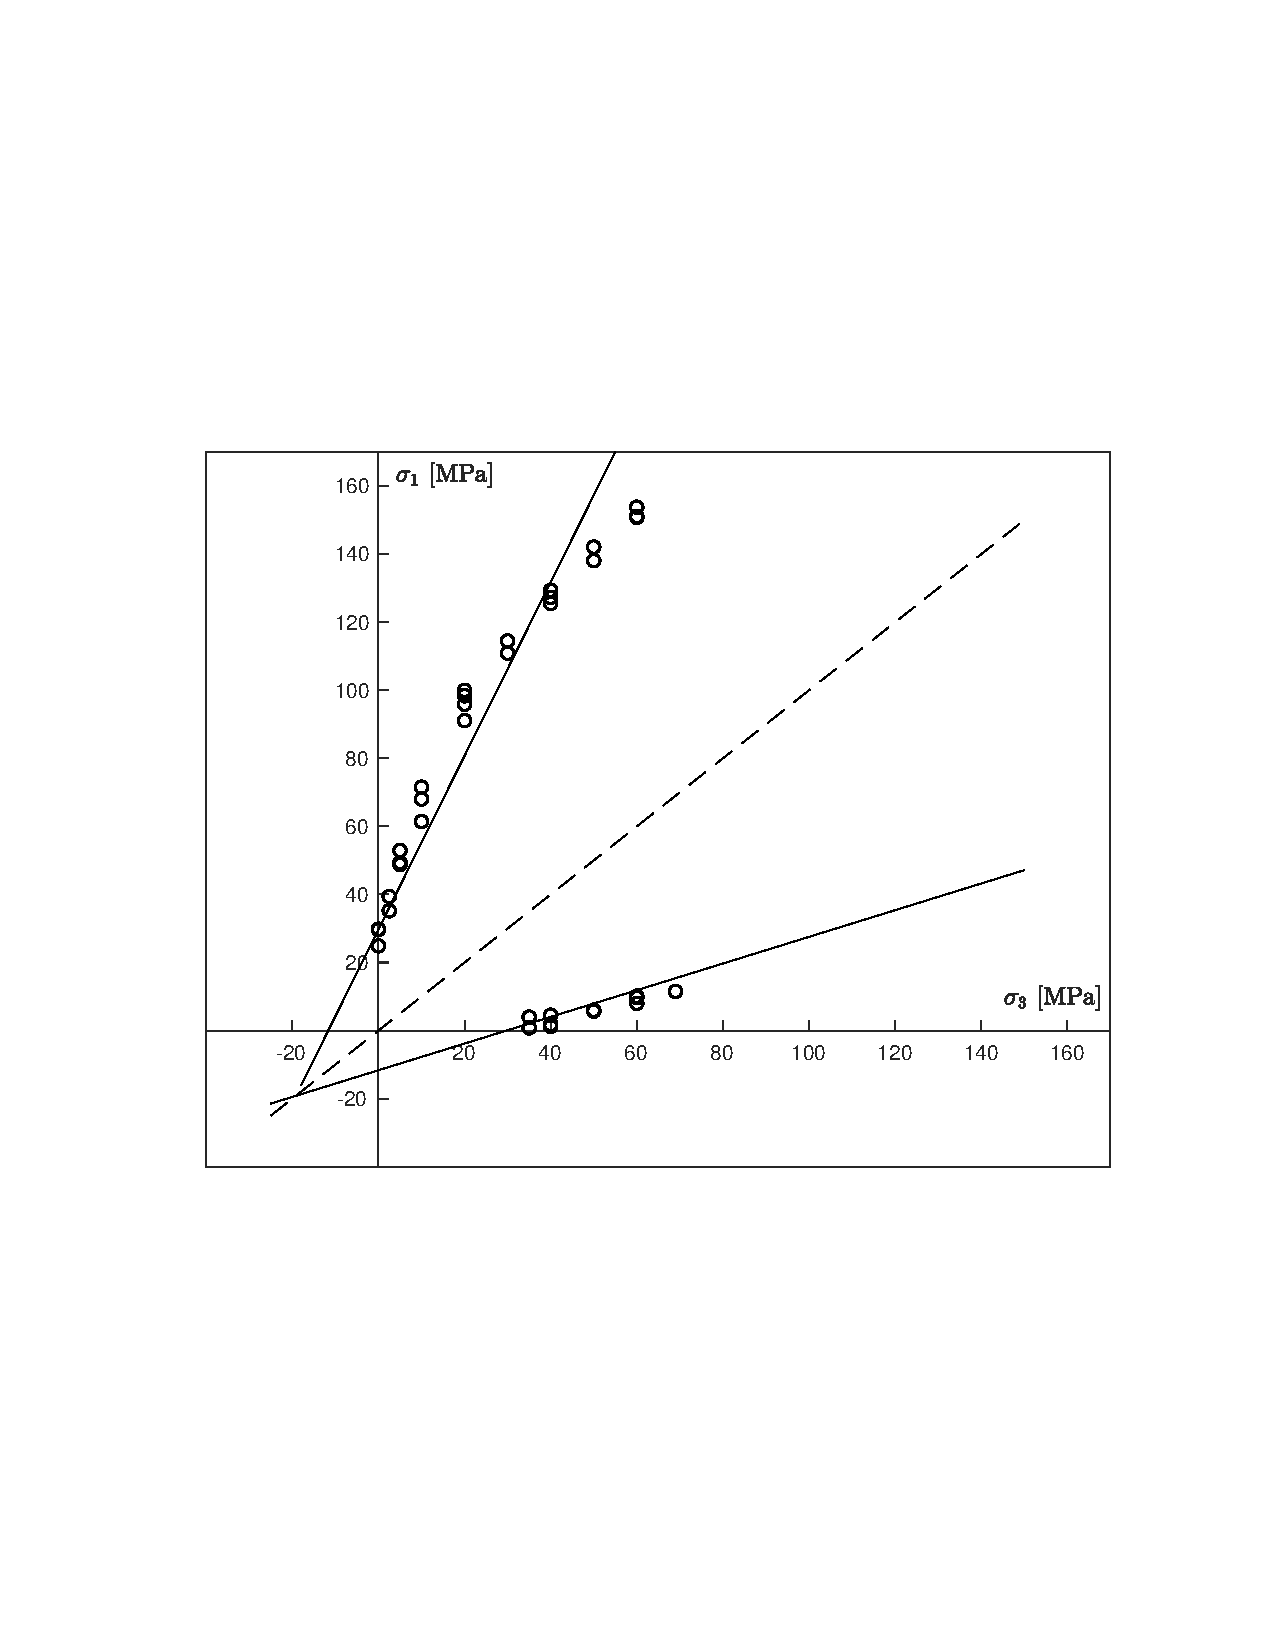
\includegraphics[width=\columnwidth]{ch2/mc_sig1sig3}
    \caption{Mohr-Coulomb criterion failure surface in  $(\sigma_3 -\sigma_1)$ plane}
    \label{fig2:mc_sig1sig3}
\end{figure}

As MC doesn’t take into account the intermediate stress effect, it can only be representative of data from conventional triaxial tests which are defined by:

Conventional Triaxial Compression (CTC): 

\begin{align*}
    \sigma_I = \sigma_1 = \sigma_a \\
    \sigma_{III} = \sigma_3 = \sigma_r\\
    \sigma_{II} = \sigma_{III} = \sigma_3 = \sigma_r
\end{align*}

Conventional Triaxial Extension (CTE):

\begin{align*}
    \sigma_I = \sigma_3 = \sigma_r \\
    \sigma_{III} = \sigma_1 = \sigma_a\\
    \sigma_{II} = \sigma_{I} = \sigma_3 = \sigma_r
\end{align*}

\subsection{Mohr-Coulomb in the \texorpdfstring{$(p - q)$}{p - q} plane} \label{ch2:MC-pq}

The following development of the MC criterion is presented for CTC and can be adapted to CTE stress definition. Following CTC stress path, Equations \ref{eq2:peq} and \ref{eq2:qeq} can be written as: 

\begin{align}
    p &= \frac{\sigma_a+2\sigma_r}{2} \label{eq2:p2} \\
    q &= \sigma_a - \sigma_r \label{eq2:q2}
\end{align}

By rearranging Equation \ref{eq2:MCfinalform} and including the CTC conditions, MC criterion becomes:

\begin{equation}\label{eq2:MCcrit}
    \sigma_a - \sigma_r = ()\sigma_a+2\sigma_r)\sin \phi + 2 \cos \phi
\end{equation}

Next equation is obtained by expanding and substituting Equation \ref{eq2:p2} and \ref{eq2:p2} in \ref{eq2:MCcrit}: 

\begin{equation}
    q(3-\sin \phi) = 6p \sin \phi + 6 \cos \phi
\end{equation}

Finally, the MC failure surface formulation in the  plane is defined by Equation \ref{eq2:q-CTC} for CTC and Equation \ref{eq2:q-CTE} for CTE:

\begin{equation}\label{eq2:q-CTC}
    q=\frac{6 \sin \phi}{3-\sin \phi} p+\frac{6 \operatorname{ccos} \phi}{3-\sin \phi} 
\end{equation}

\begin{equation}\label{eq2:q-CTE}
    q=\frac{6 \sin \phi}{3+\sin \phi} p+\frac{6 c \cos \phi}{3+\sin \phi}
\end{equation}

or in the condensed form: 

\begin{equation}
    q = m_{c,e} p + b_{c,e}
\end{equation}

where $c$ and $e$  defines $m$ and $b$ for compression or extension surfaces:

\begin{equation}\label{eq2:MC_mc_q}
    m_c=\frac{6 \sin \phi}{3-\sin \phi} 
\end{equation}
\begin{equation}\label{eq2:MC_me_q}
    m_e=\frac{6 \sin \phi}{3+\sin \phi} 
\end{equation}
\begin{equation}\label{eq2:MC_bc_q}
    b_c=\frac{6 c \cos \phi}{3-\sin \phi}
\end{equation}
\begin{equation}\label{eq2:MC_be_q}
    b_e=\frac{6 c \cos \phi}{3+\sin \phi}
\end{equation}

Fig. \ref{fig2:mc_pq} present the graphical construction of the failure surfaces in the  $(p-q)$plane. In order to distinguish compression from extension data, the failure surface in extension is showed using a negative deviatoric stress $-q$. 


\begin{figure}[tb]
    \centering
    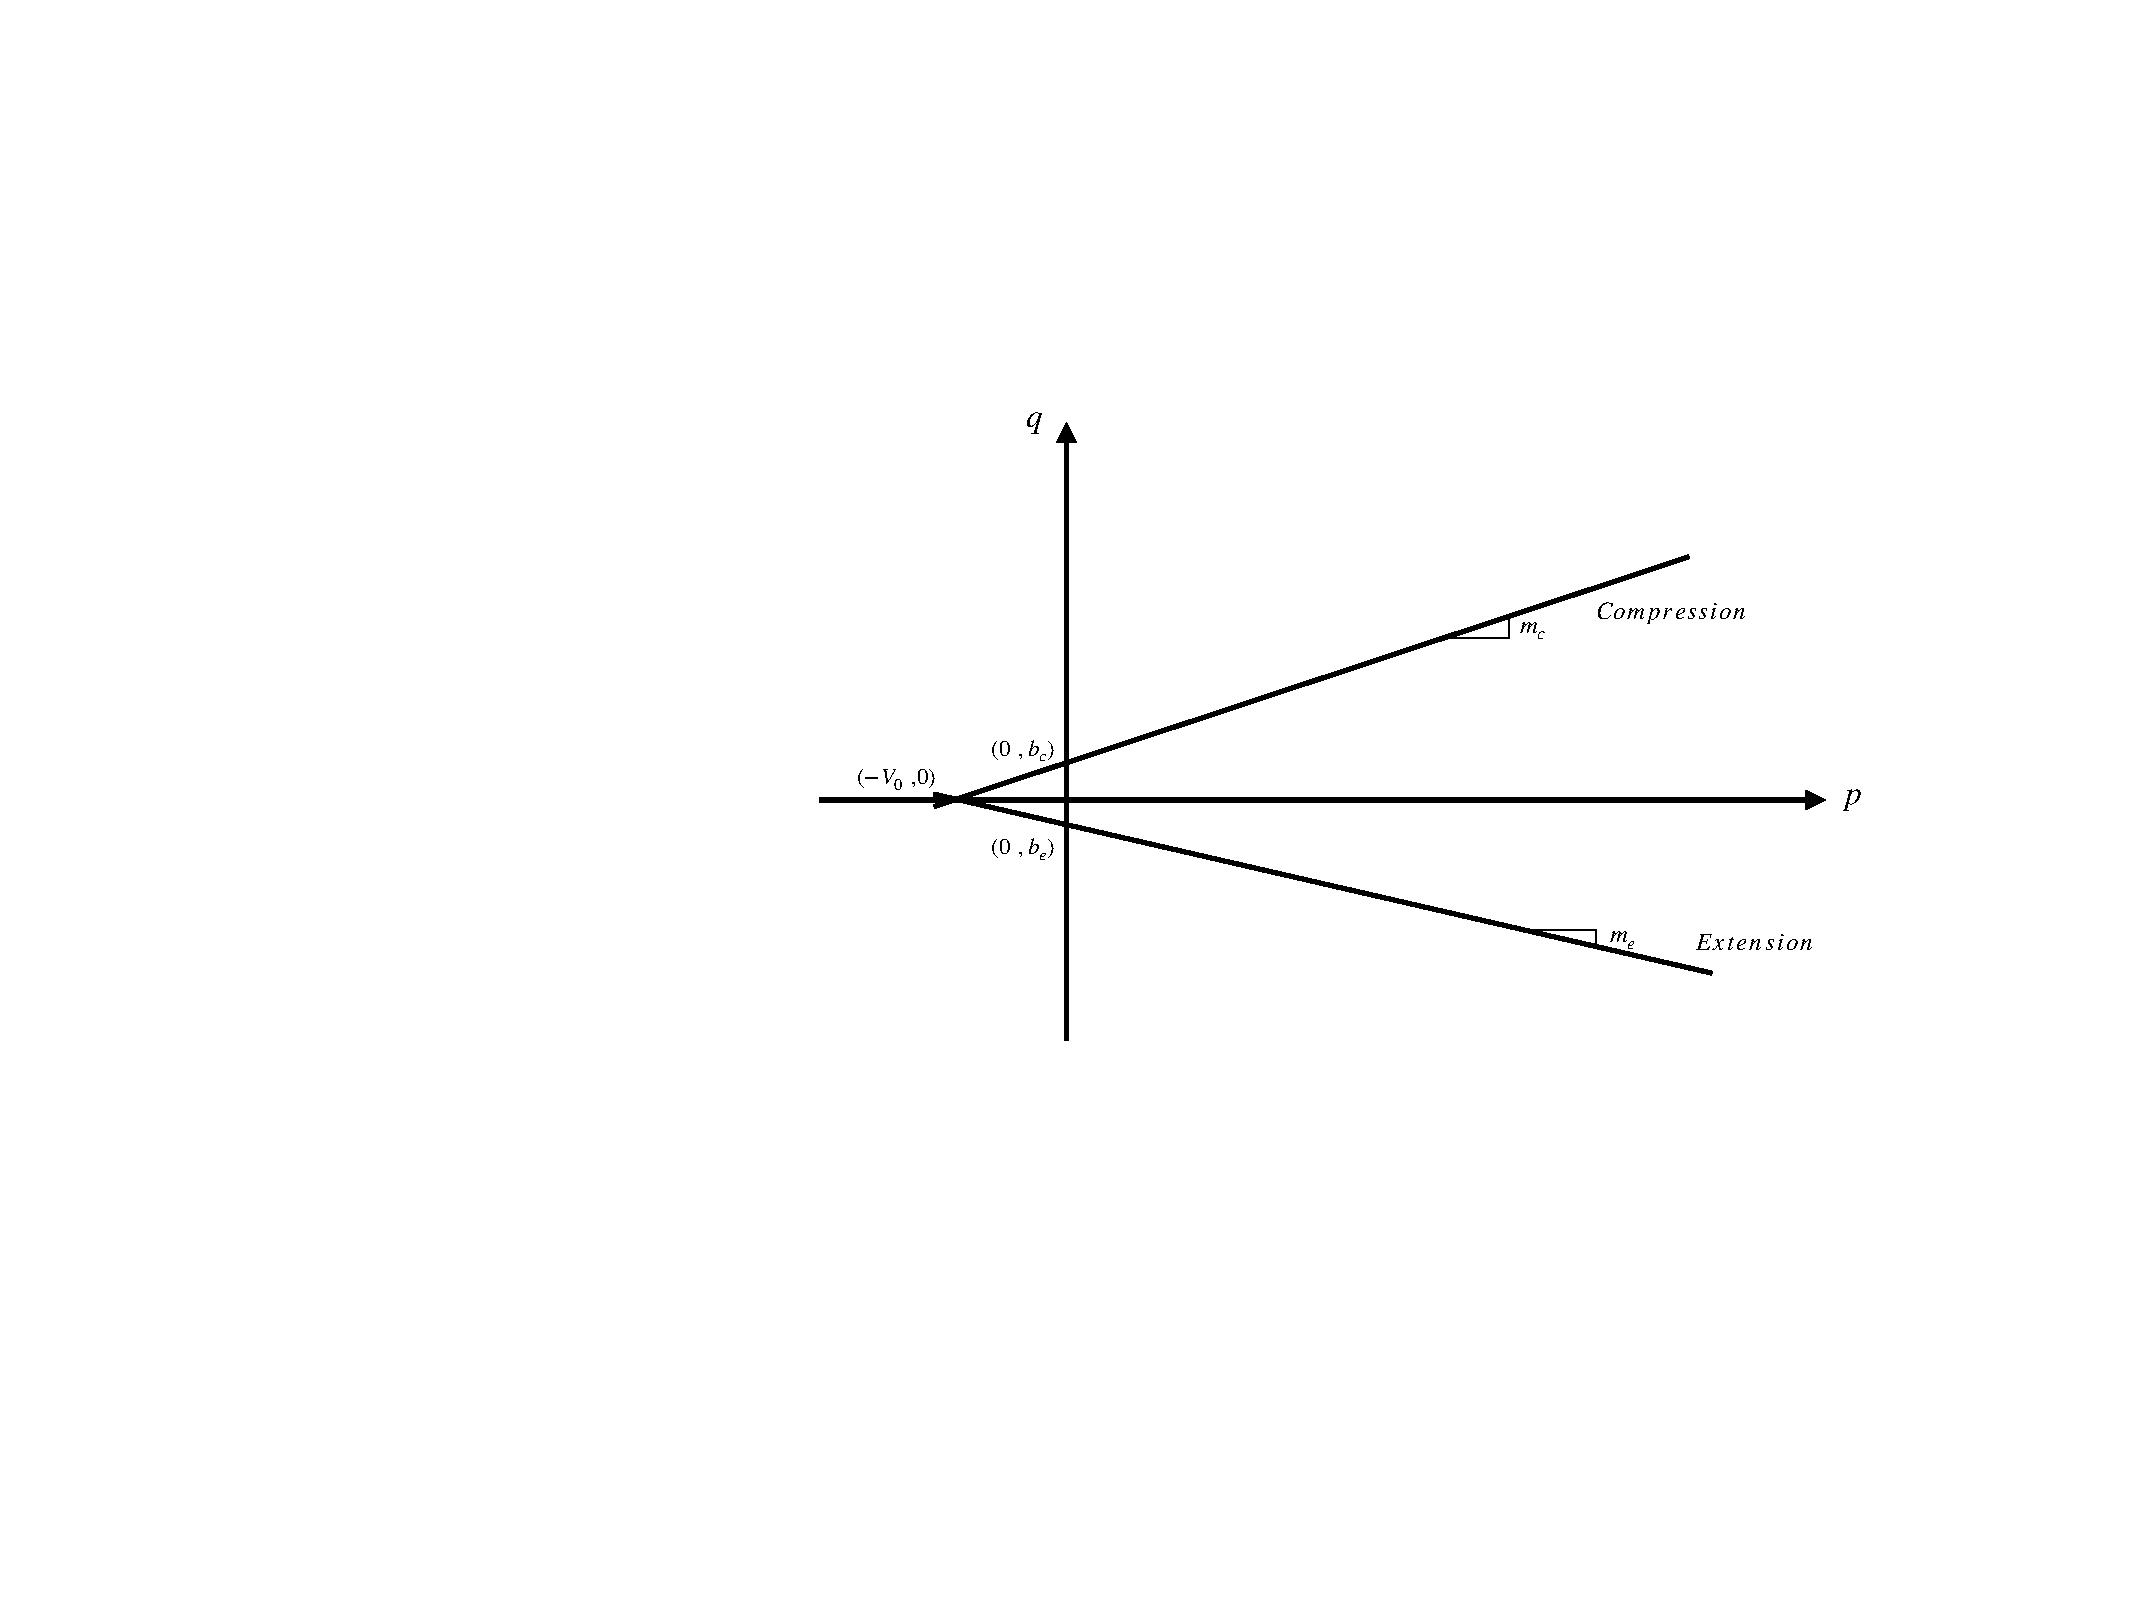
\includegraphics[width=\columnwidth]{ch2/mc_pq}
    \caption{Schematic representation of Mohr-Coulomb criterion failure surface in  $(p-s)$plane}
    \label{fig2:mc_pq}
\end{figure} 

\subsection{Mohr-Coulomb in the \texorpdfstring{$\pi$}{pi}-plane}\label{ch2:MC_pi}

The Mohr-Coulomb failure envelop in the $\pi$-plane is presented in Fig \ref{fig2:mc_pi}. The failure surfaces can be obtained by inserting Equation \ref{eq2:sig1} and \ref{eq2:sig3} in the criterion formulation defined by \ref{eq2:MCcondenseform}. 

\begin{figure}[tb]
    \centering
    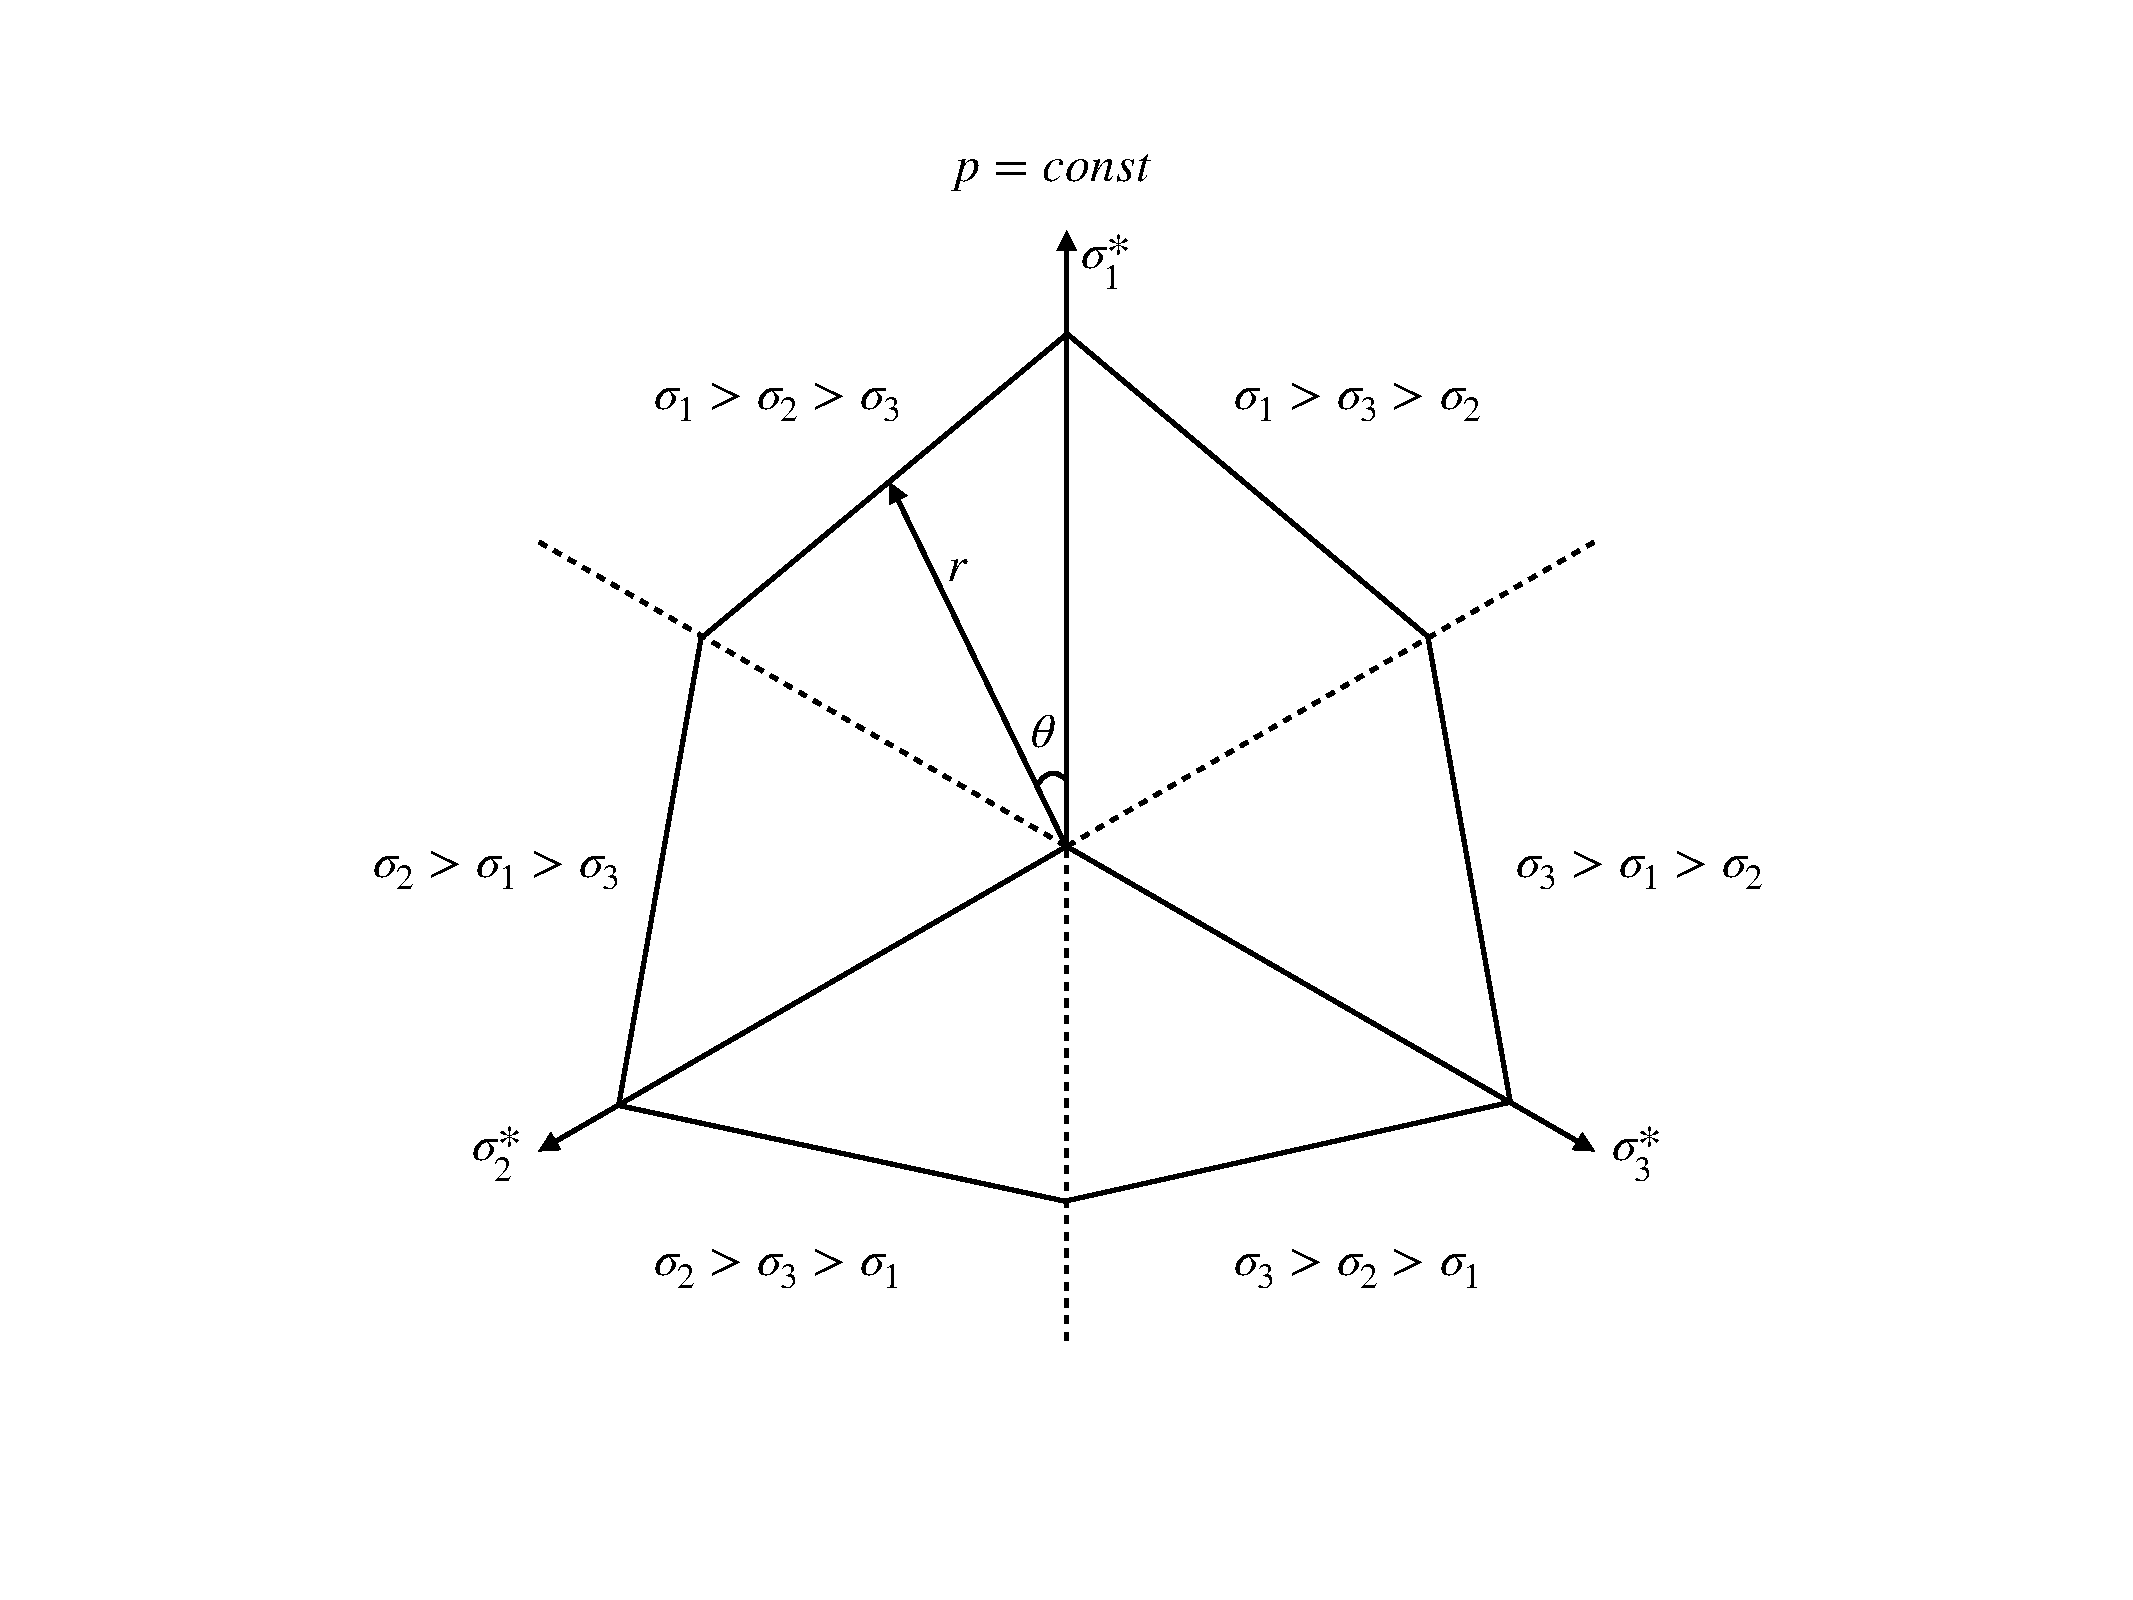
\includegraphics[width=\columnwidth]{ch2/mc_pi}
    \caption{Schematic representation of Mohr-Coulomb criterion failure surface in  $\pi$plane}
    \label{fig2:mc_pi}
\end{figure} 

\section{Hoek-Brown criterion}

The Hoek-Brown (HB) criterion is a non-linear criterion for isotropic rocks that doesn’t take into account the intermediate stress effect. The empirical relationship developed between the principal stresses can be written as follow:

\begin{equation}\label{eq2:HC-crit}
    \sigma_{I}=\sigma_{I I I}+C_{0} \sqrt{m \frac{\sigma_{I I I}}{C_{0}}+s}
\end{equation}

Hoek and Brown (1980) \cite{Hoek1980} define $m$ and $s$  are constant depending on the rock properties. The constant $s$ characterize the initial state of the tested rock: for intact rock $s=1.0$. This value will be considered in the next developments. The strength parameter $m$ is an empirical fitting parameter chosen depending on the rock type. 

\subsection{Hoek-Brown in the \texorpdfstring{$(\sigma_3 -\sigma_1)$}{sigma 3 - sigma 1} plane}

For conventional triaxial compression, the conditions presented in section \ref{ch2:MC-pq} can be inserted in Equation \ref{eq2:HC-crit} to obtain the criterion formulation in terms of the axial and radial stresses:

\begin{equation}\label{eq2:HBsig1}
    \sigma_{1}=\sigma_{3}+C_{0} \sqrt{m \frac{\sigma_{1}}{C_{0}}+1}
\end{equation}

Similarly, the formulation for conventional triaxial extension is written as:

\begin{equation}
    \sigma_{1}=\sigma_{3} - \frac{\sqrt{4 m C_{0} \sigma_{3}+m^{2} C_{0}^{2}+4 C_{0}^{2}}-m C_{0}}{2}
\end{equation}

From Equation \ref{eq2:HBsig1} (2.28), the theoretical isotropic tensile strength $V_0$ can be expressed as a function of the uniaxial compression strength $C_0$, using : $\sigma_a = \sigma_r = -V_0$:

\begin{equation}
    V_0 = \frac{C_0}{m}
\end{equation}

Fig. \ref{fig2:hb_sig1sig3} present the HB failure surfaces in the $(\sigma_3 -\sigma_1)$ plane. 

\begin{figure}[tb]
    \centering
    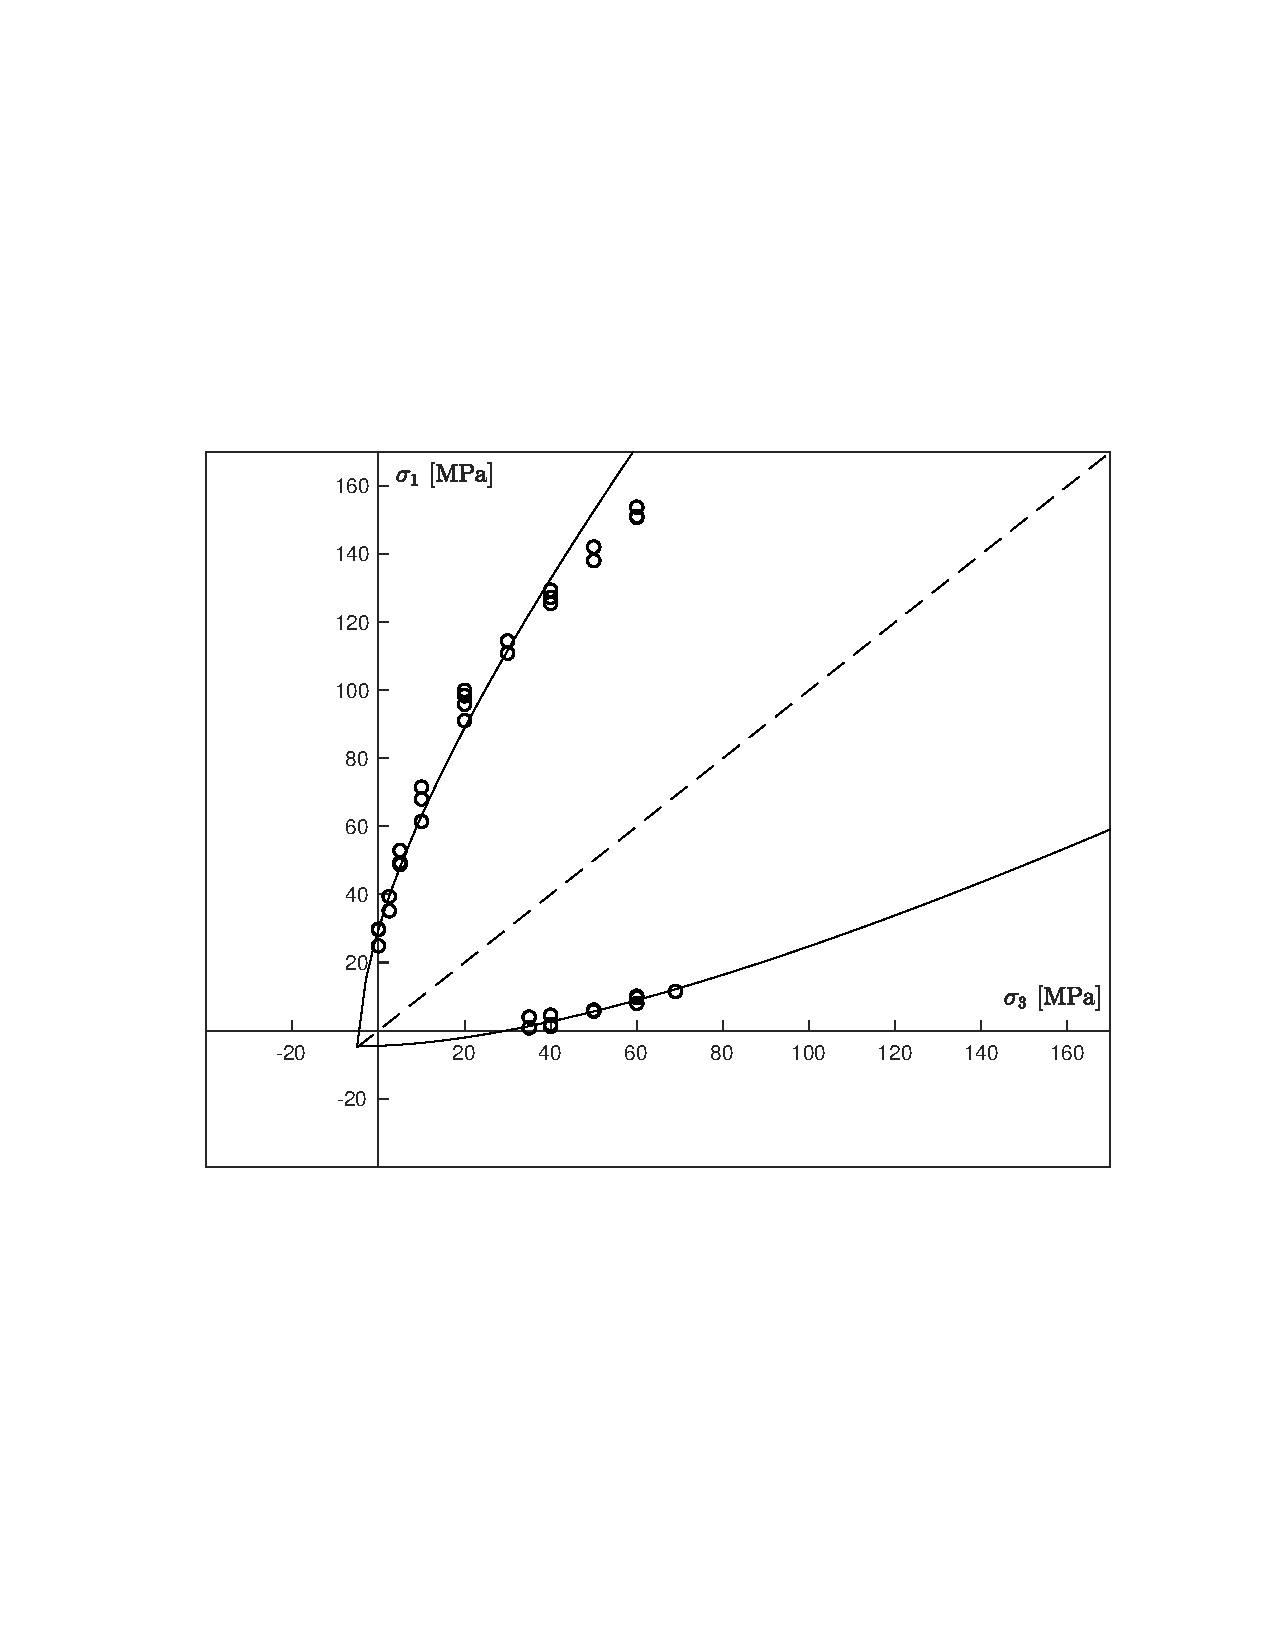
\includegraphics[width=0.8\columnwidth]{ch2/hb_sig1sig3}
    \caption{Schematic representation of Hoek-Brown criterion failure surface in $(\sigma_3 -\sigma_1)$ plane.}
    \label{fig2:hb_sig1sig3}
\end{figure} 

\subsection{Hoek-Brown in the \texorpdfstring{$(p-q)$}{p-q} plane}

HB criterion can be expressed with the stress invariants  and . By rearranging Equation\ref{eq2:HBsig1} (2.27) the formulation become:

\begin{equation}\label{eq2:HB-crit-pq}
    \left(\sigma_{I}-\sigma_{I I I}\right)^{2}=C_{0}^{2}\left(m \frac{\sigma_{I I}}{C_{0}}+s\right)
\end{equation}

By rearranging and inserting $p$  and $q$ in Equation \ref{eq2:HB-crit-pq} (2.31), implicit formulation for CTC and CTE are obtained. Equation \ref{eq2:HB-q-CTC} for compression and \ref{eq2:HB-q-CTE} for extension describe HB criterion after solving roots of the implicit expressions:  


\begin{align}
    q&=\frac{1}{6}\left(\pm \sqrt{C_{0}} \sqrt{C_{0} m^{2}+36 C_{0}+36 m p}-C_{0} m\right) \label{eq2:HB-q-CTC} \\
    q&=\frac{1}{3}(\pm \sqrt{\left.C_{0}^{2} m^{2}+9 C_{0}^{2}+9 C_{0} m p+C_{0} m\right)} \label{eq2:HB-q-CTE}
\end{align}

The HB criterion surface fitting in the  plane is presented in Fig \ref{fig2:hb_pq}, where the positive root of Equation \ref{eq2:HB-q-CTC} and the negative root of Equation \ref{eq2:HB-q-CTE} are considered.

\begin{figure}[tb]
    \centering
    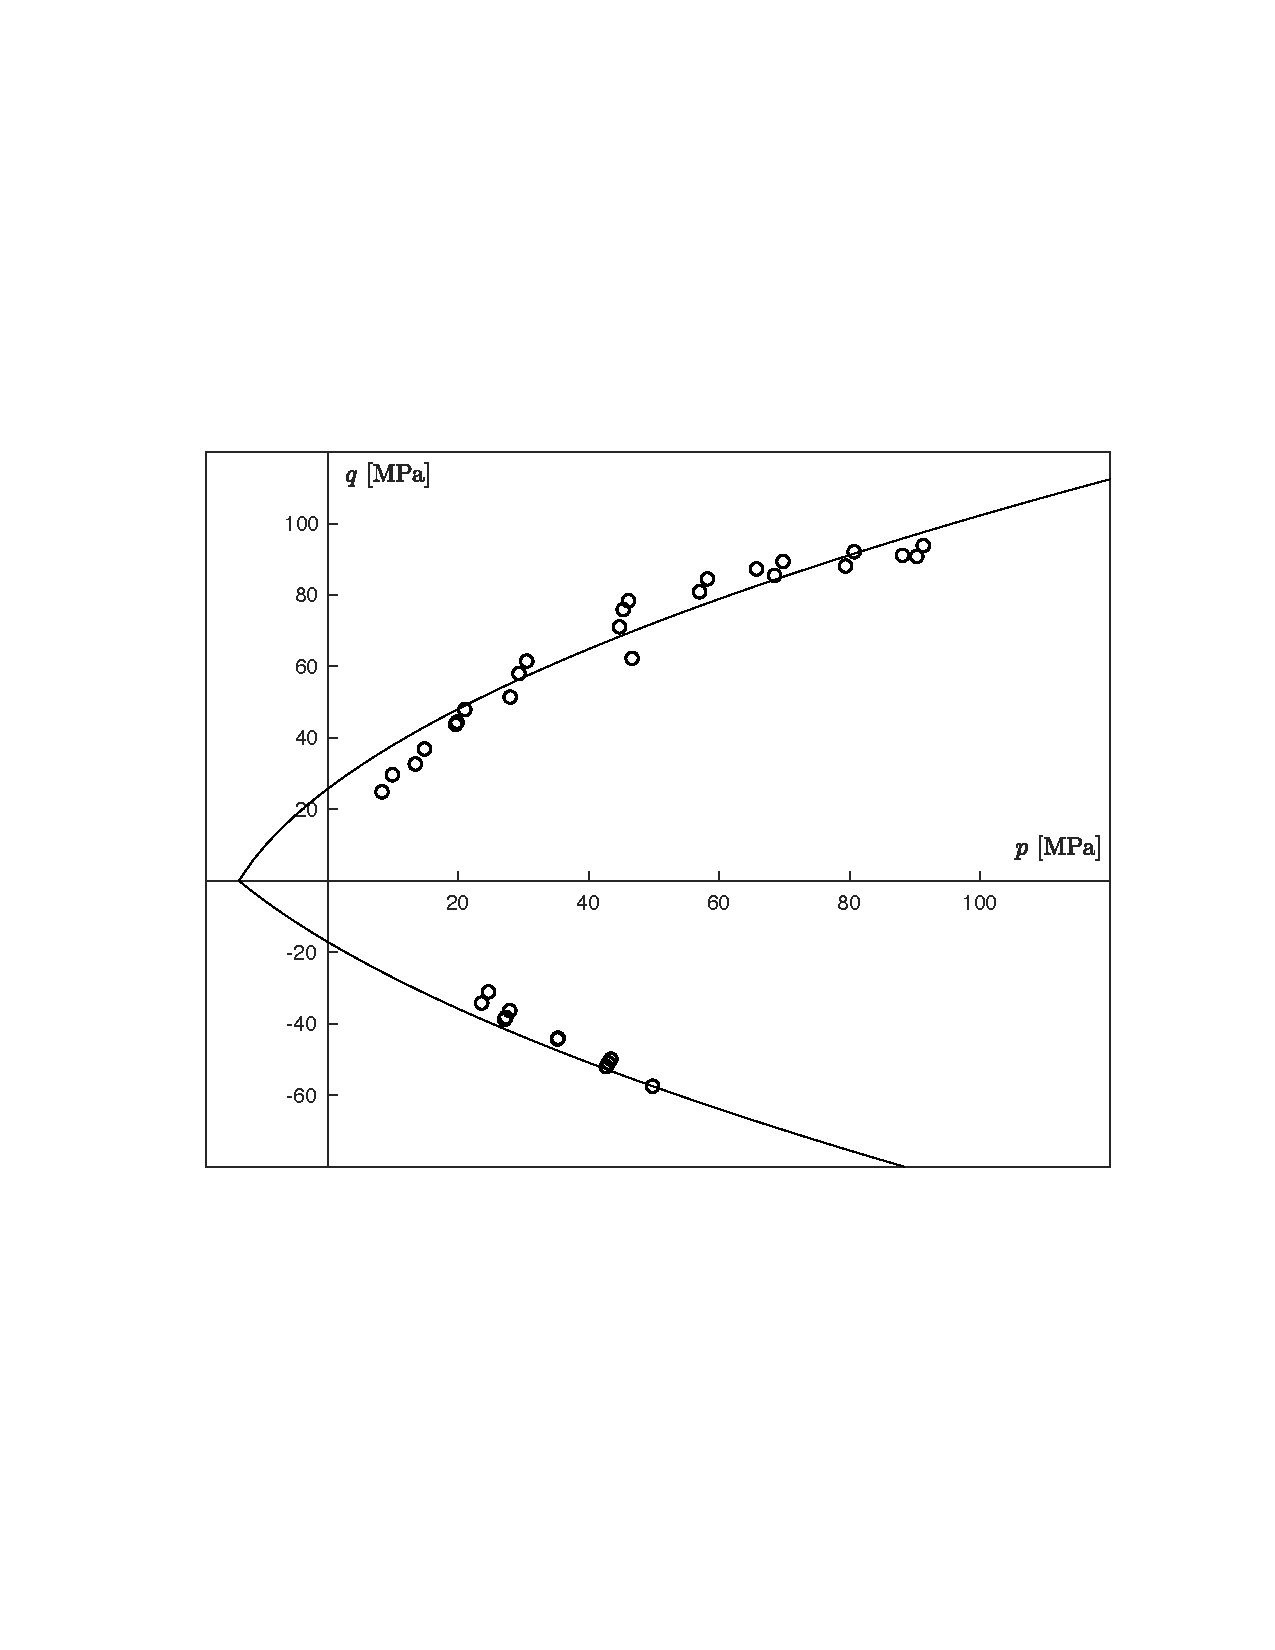
\includegraphics[width=\columnwidth]{ch2/hb_pq}
    \caption{Schematic representation of Hoek-Brown criterion failure surface in $(p-q)$ plane.}
    \label{fig2:hb_pq}
\end{figure} 

\subsection{Hoek-Brown in the \texorpdfstring{$\pi$}{pi} plane}

The Hoek-Brown failure envelop in the -plane is presented in Fig \ref{fig2:hb_pi} The failure surfaces can be obtained by inserting Equation \ref{eq2:sig1} (2.11) and \ref{eq2:sig3}  (2.13) in the criterion formulation defined by \ref{eq2:HC-crit}. In Fig 7, the surfaces are exaggerated to show the non-linearity of the criterion.  

\begin{figure}[tb]
    \centering
    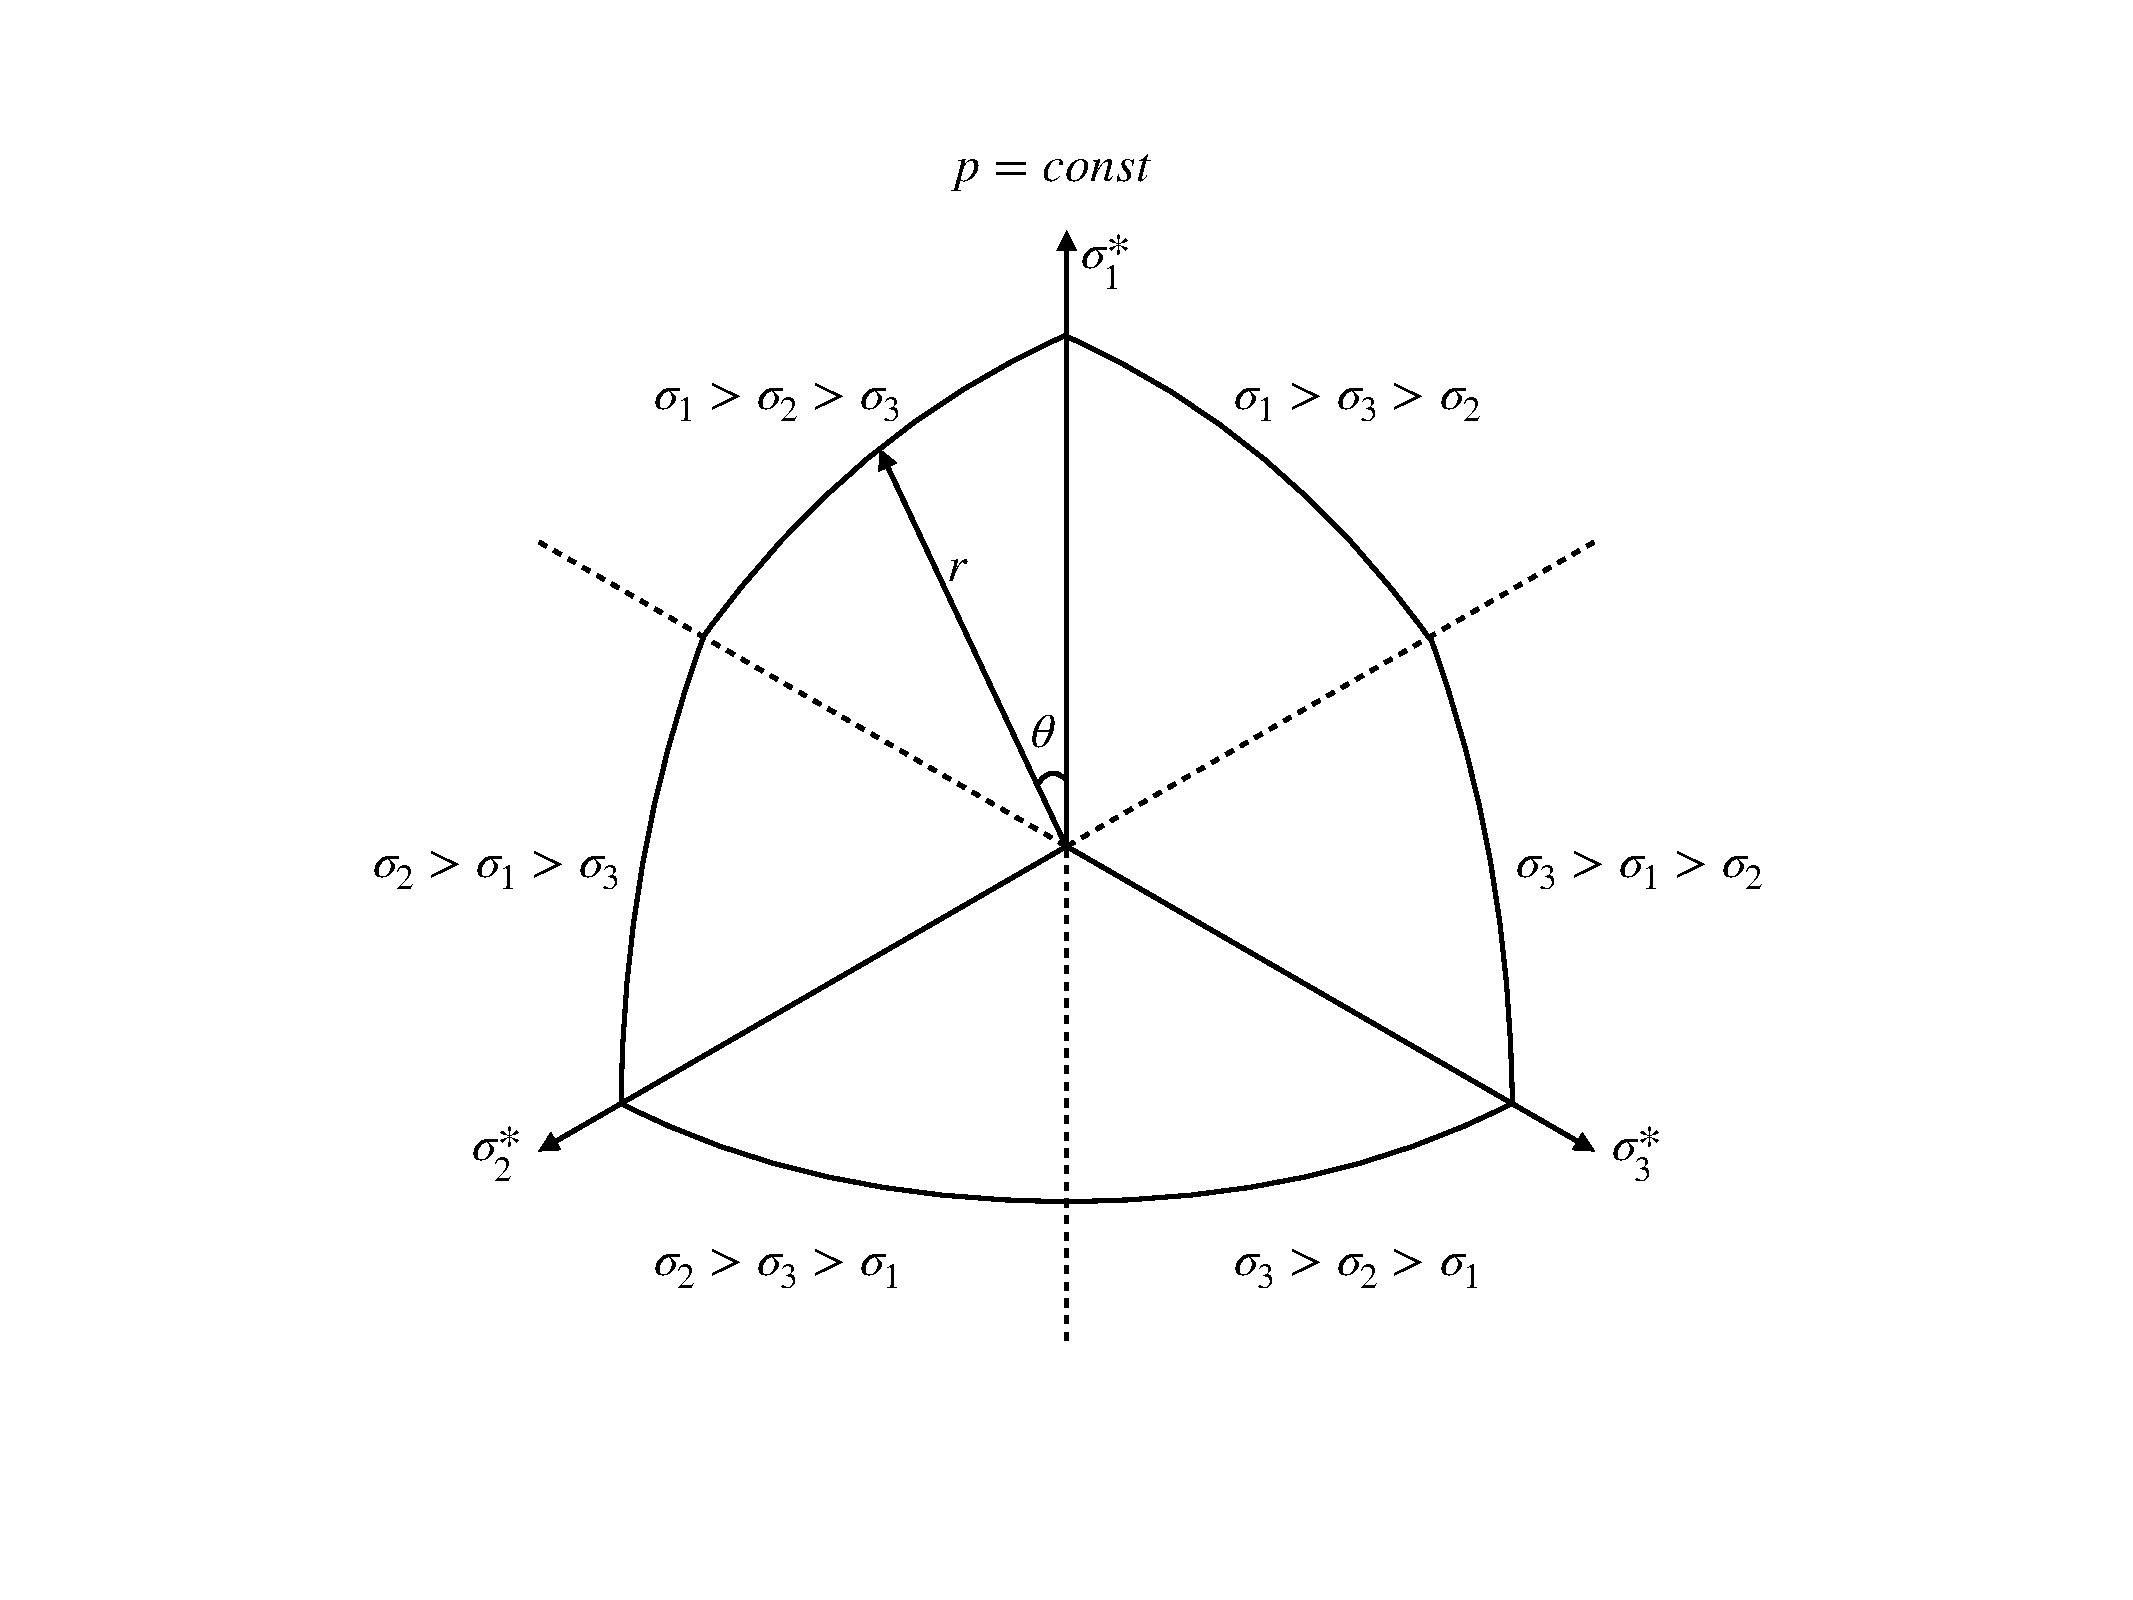
\includegraphics[width=\columnwidth]{ch2/hb_pi}
    \caption{Schematic representation of Hoek-Brown criterion failure surface in $\pi$ plane.}
    \label{fig2:hb_pi}
\end{figure} 

\section{Paul-Mohr-Coulomb criterion}

The Paul-Mohr-Coulomb criterion (PMC) is a linear criterion formulated in terms of the three principal stresses. Unlike the Mohr-Coulomb and Hoek-Brown, PMC is representative of all multi-axial experiments. Its formulation is based on the one developed by Mohr-Coulomb, for which the intermediate stress effect is added \cite[Paul (1968)]{Paul1968}). 

PMC failure criterion have the following general expression:

\begin{equation}\label{eq2:PMC}
    A\sigma_I + B\sigma_{II}+C\sigma_{III} = 1
\end{equation}

The ordering of the $A$, $B$ and $C$ with the major, intermediate and minor stresses should be kept as defined in Equation \ref{eq2:PMC}. 

In their work, \cite[Meyer and Labuz (2013)]{Meyer2013} provides the expression of the coefficient ,  and  in terms of the rock properties:

\begin{align}
    A &= \frac{1-\sin \phi_c}{2V_0\sin \phi_c} \\
    B &= \frac{\sin \phi_c - \sin \phi_e}{2V_0 \sin \phi_e \sin \phi_c} \\
    C &= \frac{-1+\sin \phi_e}{2V_0\sin \phi_e} \\
\end{align}

Equation \ref{eq2:PMC} can therefore be written in its complete form as follow:

\begin{equation}\label{eq2:PMCsin}
    \sigma_{I}\left[\frac{1-\sin \phi_{c}}{2 V_{0} \sin \phi_{C}}\right]+\sigma_{I}\left[\frac{\sin \phi_{c}-\sin \phi_{e}}{2 V_{0} \sin \phi_{e} \sin \phi_{C}}\right]+\sigma_{I I I}\left[\frac{-1+\sin \phi_{e}}{2 V_{0} \sin \phi_{e}}\right]=1
\end{equation}

PMC refines failure criterion definition by considering different values of the rock properties.  It is shown in Equation \ref{eq2:PMCsin} by the subscripts $c$ and $e$, defining the variables for compression or extension.

\subsection{Paul-Mohr-Coulomb in the \texorpdfstring{$(\sigma_3 -\sigma_1)$}{sigma 3 - sigma 1} plane}\label{ch2:PMCsig1sig3}

Paul-Mohr-Coulomb is a “involved” version of the Mohr-Coulomb criterion, therefore its expression in the  $(\sigma_3 -\sigma_1)$plane is an adjustment of Equation \ref{eq2:PMCsin} considering different friction angles and cohesion for compression and extension conditions: 

\begin{equation}
    \sigma_I = M_{c,e}\sigma_{III}+C{c,e}
\end{equation}

Where:

\begin{equation}
    M_{c,e} = \frac{1+\sin \phi_{c,e}}{1-\sin \phi_{c,e}}
\end{equation}

\begin{equation}
    C_{c,e} = \frac{2c_{c,e}\cos \phi_{c,e}}{1-\sin \phi_{c,e}}
\end{equation}

PMC failure surfaces in $(\sigma_3 -\sigma_1)$ plane are presented in Fig. \ref{fig2:pmc_sig1sig3}. As the friction angle and the cohesion for compression and extension are non-equal, PMC isn’t symmetrical over the hydrostatic axis. The computation $V_0$ of  will be discussed in section \ref{ch2:pmcfit}. 


\begin{figure}[tb]
    \centering
    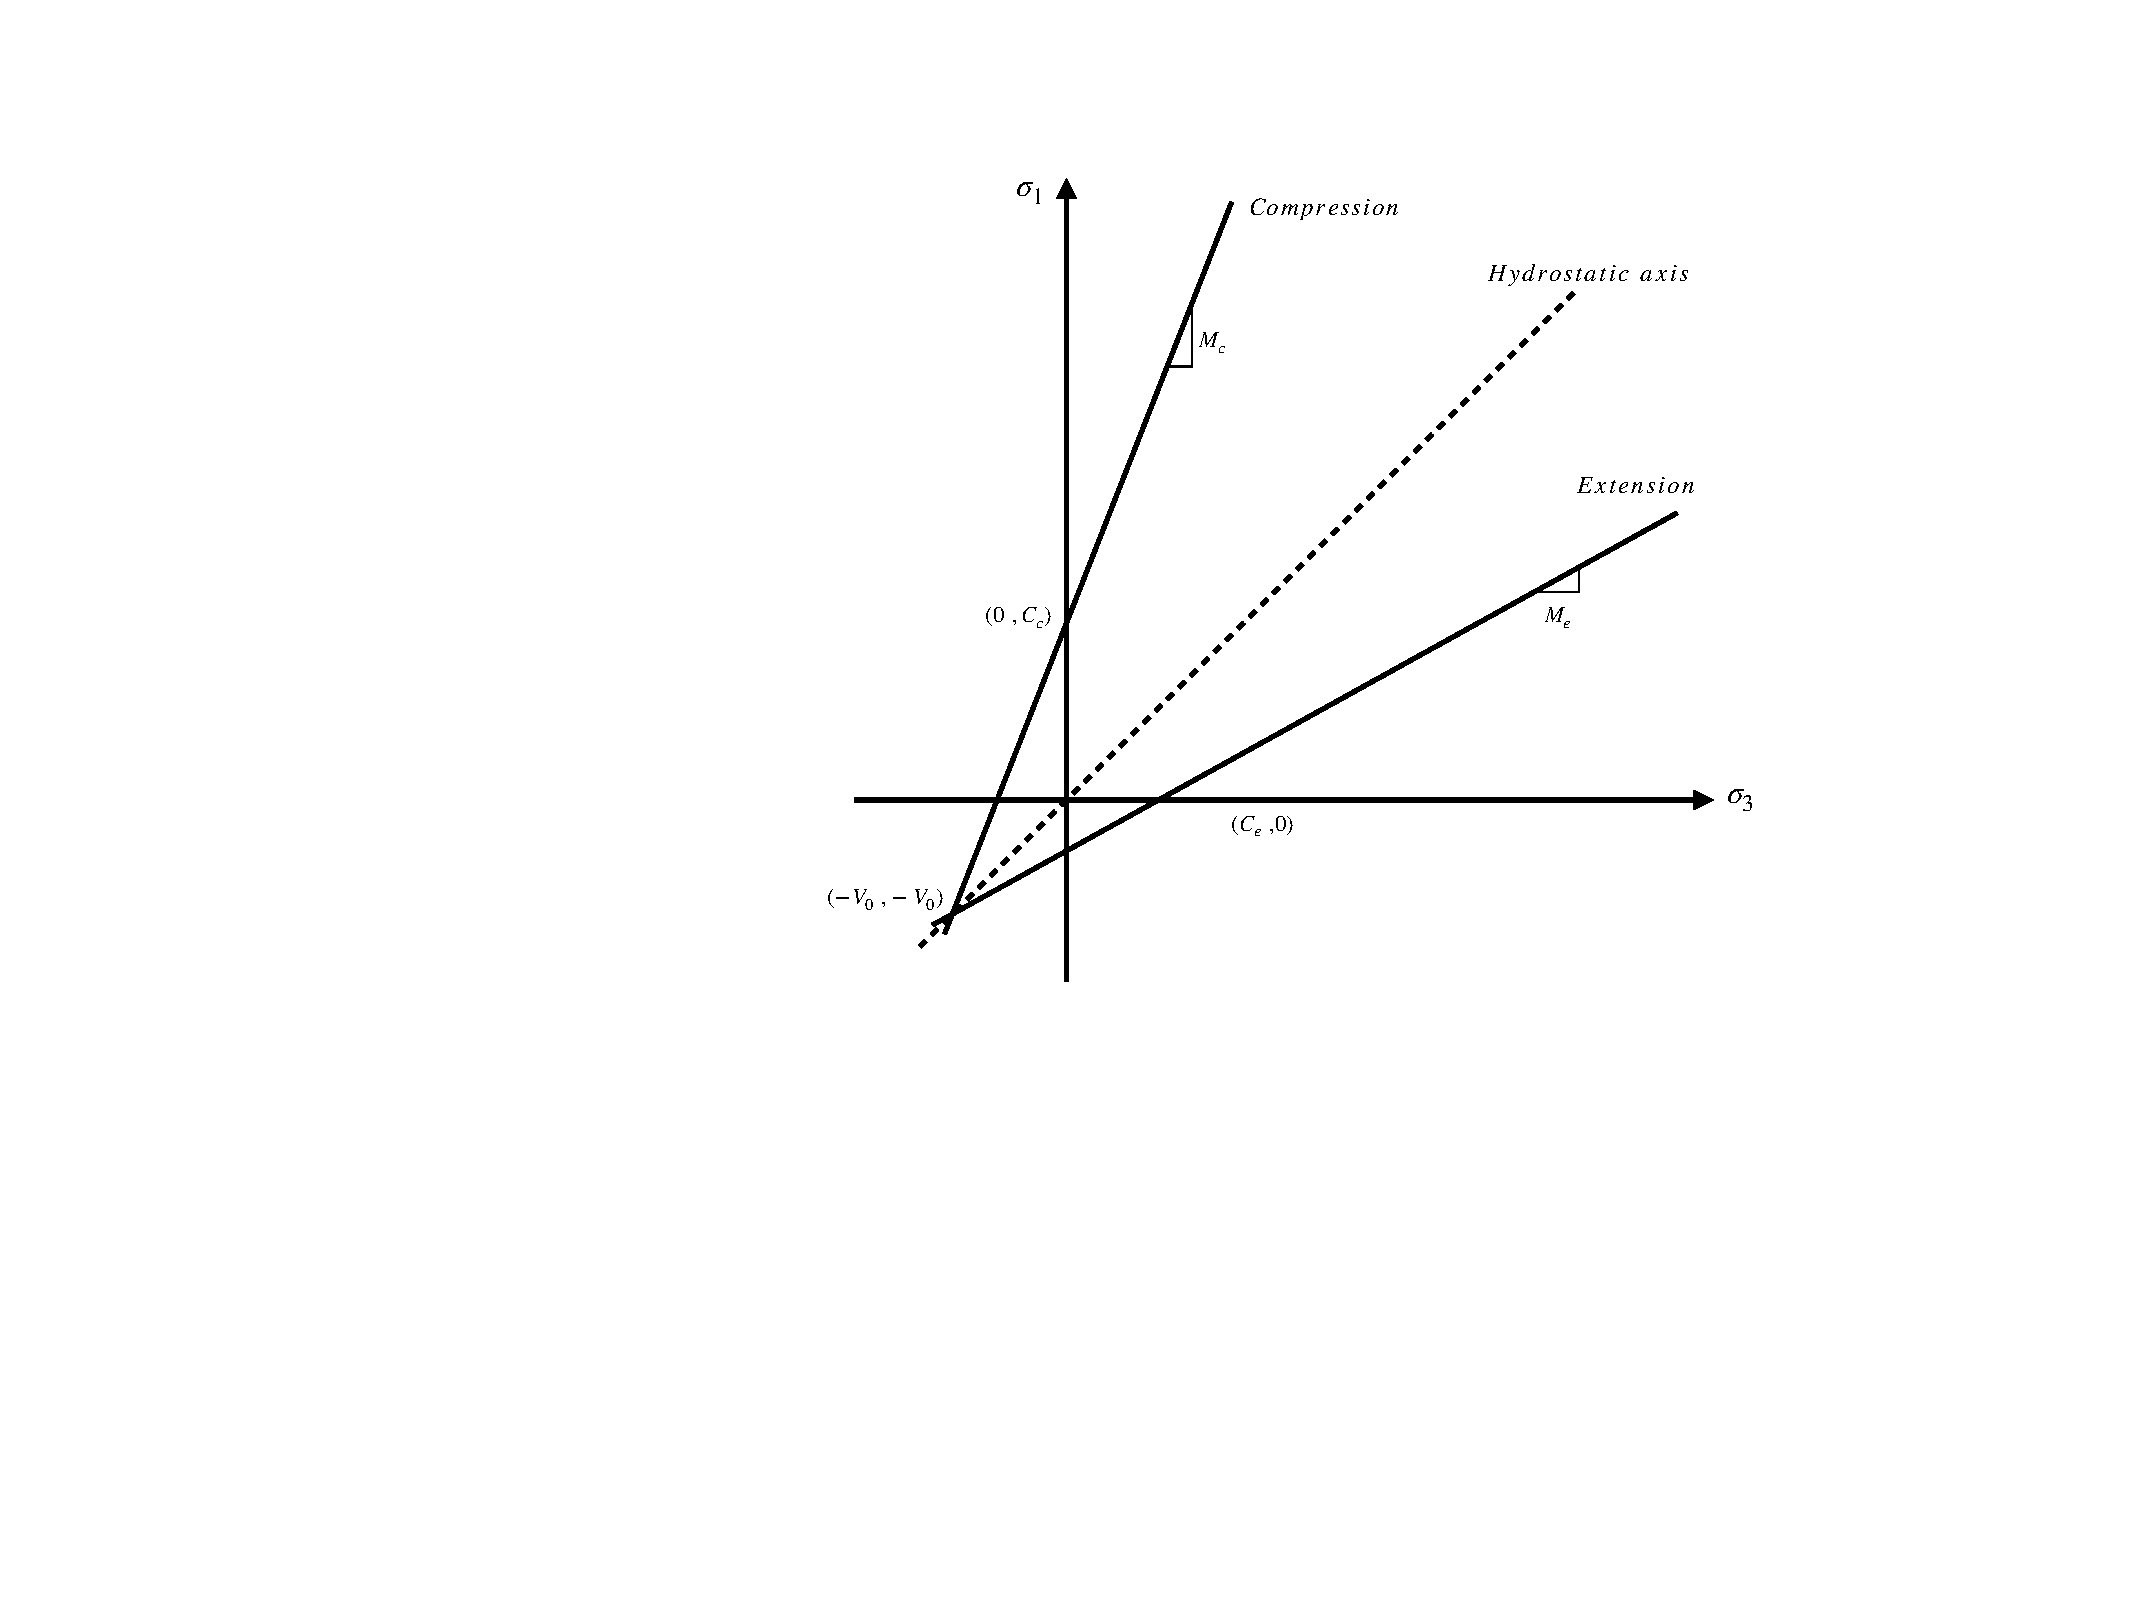
\includegraphics[width=\columnwidth]{ch2/pmc_sig1sig3}
    \caption{Schematic representation of Paul-Mohr-Coulomb criterion failure surface in $(\sigma_3 -\sigma_1)$ plane.}
    \label{fig2:pmc_sig1sig3}
\end{figure} 

\subsection{Paul-Mohr-Coulomb in the \texorpdfstring{$(p-q)$}{p-q} plane}

To represent PMC in the  plane, an adjusted version of Equations \ref{eq2:q-CTC} and \ref{eq2:q-CTE} defined for MC can be used:

\begin{equation}\label{eq2:pmc-q-CTC}
    q=\frac{6 \sin \phi_{c}}{3-\sin \phi_{c}} p+\frac{6 c_{c} \cos \phi_{c}}{3-\sin \phi_{c}}
\end{equation}

\begin{equation}\label{eq2:pmc-q-CTE}
    q=\frac{6 \sin \phi_{e}}{3+\sin \phi_{e}} p+\frac{6 \operatorname{ccos} \phi_{e}}{3+\sin \phi_{e}}
\end{equation}

or in the simplifies form:

\begin{equation}
    q = m_{c,e}p+b{c,e}
\end{equation}

The same sketch of the failure surface as presented in Fig. \ref{fig2:mc_pq} for Mohr-Coulomb can be used to represent Paul-Mohr-Coulomb criterion. The only difference is the non-equal values of the friction angles and cohesions in the computation of $m_{c,e}$ and $b_{c,e}$.

\subsection{Paul-Mohr-Coulomb fitting }\label{ch2:pmcfit}

Failure criterion are conjectural. They try to provide a mathematical formulation of rock behavior based on experiments. However, the results obtained from them aren’t direct measurements of the friction angle or cohesion, they give the state of stress at failure. The rock properties should then be computed from these stresses.

Failure criterion fitting consist in the computation of the rock properties ($V_0$, $\phi$, $c$ ) from a mathematical formulation of the criterion written in terms of the three principal stresses. Labuz (2018) \cite{Labuz2018} and Folta (2016) \cite{Folta2016} provide detailed mathematical derivation of Equations \ref{eq2:sig1} - \ref{eq2:sig3} that leads to the expression of Paul-Mohr-Coulomb failure criterion in terms of the stress invariants $p$, $q$  and $\theta$. 

The final formulation is given by Equation \ref{eq2:PMCfinalform}:

\begin{equation}\label{eq2:PMCfinalform}
    q\cos(\phi) = \frac{b_c}{V_0}p+k\sin(\phi)q+b_c
\end{equation}

where:

\begin{align}
    k &= \frac{1-2\alpha }{\sqrt{3}}\\
    \alpha &= \frac{b_c}{b_e}
\end{align}

Each data point $i$ from a conventional triaxial or multi-axial experiment is defined by a trio of $(p_i,q_i,\theta_i)$ values. Therefore, for one tested rock, Equation \ref{eq2:PMCfinalform} describes a system of linear equations. This system has $m$  equations, with $m$ being the number of experiments performed on the considered rock. Equation \ref{eq2:PMCfinalform} can also be written as a matrix equation of type $Ax=b$ :

\begin{equation}\label{eq2:mat-eq}
    \left[\begin{array}{c}
    {q_{1} \cos \left(\theta_{1}\right)} \\
    {\cdots} \\
    {q_{m} \cos \left(\theta_{m}\right)}
    \end{array}\right]=\left[\begin{array}{ccc}
    {p_{1}} & {q_{1} \sin \theta_{1}} & {1} \\
    {\cdots} & {\cdots} & {\cdots} \\
    {p_{m}} & {q_{m} \sin \theta_{m}} & {1}
    \end{array}\right]\left[\begin{array}{c}
    {b_{c} / V_{0}} \\
    {k} \\
    {b_{c}}
    \end{array}\right]
\end{equation}

with $A$ a m-by-3 matrix, $b$ a m-row vector and $x$  a 3-row vector. 

From the system defined in Equation \ref{eq2:mat-eq}, $b_c$ , $k$ and $V_0$  and can be determined. $k$ and $b_c$  are given by the second and third row of parameter vector $x$ , and $V_0$  is computed using the first row :
\begin{equation}
    V_0 = \frac{b_c}{x_1}
\end{equation}

The rock parameters can now be defined by solving Equations for \ref{eq2:pmc-q-CTC} and \ref{eq2:pmc-q-CTE} for $q=0$  and $p=-V_0$ :
\begin{align}
    \sin \phi_c &= \frac{3b_c}{6V_0+b_c} \\
    \sin \phi_e &= \frac{3b_c}{6V_0-b_e} 
\end{align}